\begin{answer}
\begin{figure}[H]
    \centering
    \begin{subfigure}{0.45\textwidth}
        \centering
        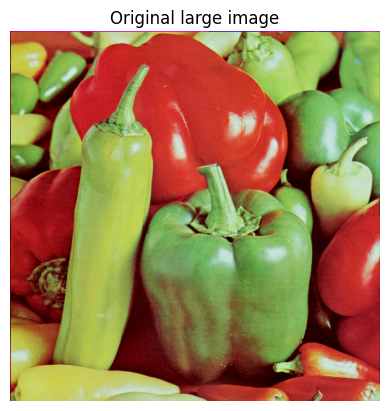
\includegraphics[width=\textwidth]{src/k_means/orig_large.png}
        \caption{Image 1}
        \label{fig:image1}
    \end{subfigure}
    \hfill
    \begin{subfigure}{0.45\textwidth}
        \centering
        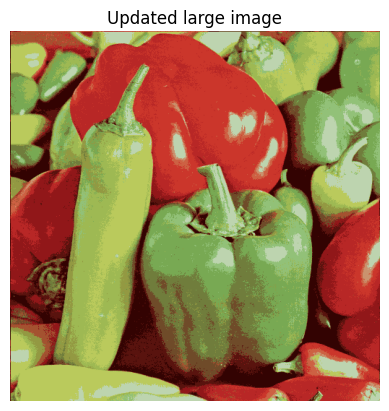
\includegraphics[width=\textwidth]{src/k_means/updated_large.png}
        \caption{Image 2}
        \label{fig:image2}
    \end{subfigure}
    \caption{Side-by-side comparison of images}
    \label{fig:comparison}
\end{figure}
\end{answer}
